\chapter{Hiukkassuodatin}%
\label{ch:dpf}



Dieselmoottorin hiukkassuodatin, eli DPF (\emph{eng. Diesel Particulate Filter}) on tehokkain järjestelmä pakokaasun noki- ja tuhkapartikkeleiden suodatukseen. 
Hyvä DPF suodattaa läpivirtaavasta pakokaasusta jopa 99\% hiukkaslukumäärästä ja 95\% -massasta \cite{Yan_state_of_the_art}. Hiukkassuodatin on osa useammasta komponentista koostuvaa jälkikäsittelyjärjestelmää, jota on havainnollistettu Kuvassa \ref{fig:EAT_full}. %Moderni jälkikäsittelyjärjestelmä koostuu yleensä hapettavasta katalysaattorista(DOC, \emph{eng. Diesel Oxidation Catalyst}), hiukkassuodattimesta (DPF),  SCR, ASC

\begin{figure}[H]
    \centering
    \pdftooltip{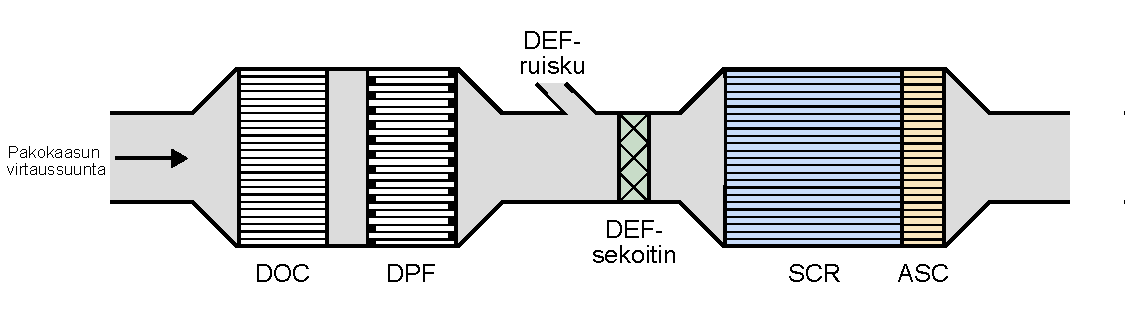
\includegraphics[width=\textwidth]{figures/EAT.pdf}}
                {Kuvituskuva hapetuskatalysaattorista ja hiukkassuodattimesta.}
    \caption{Modernin jälkikäsittelyjärjestelmän osat.}
    \label{fig:EAT_full}
\end{figure}



\section{Järjestelmän fyysinen rakenne}

Tyypillisin DPF-tyyppi on ns. seimämävirtaus-DPF (\emph{eng. wall-flow DPF}), jossa pakokaasu virtaa vuoronperään vastakkaisista päistään suljetuissa putkissa. Pakokaasu virtaa putkien välillä huokoisten seinämien läpi. Virtausta on havainnollistettu Kuvassa \ref{fig:wall-flow-dpf}  


\begin{figure}[H]
    \centering 
    \pdftooltip{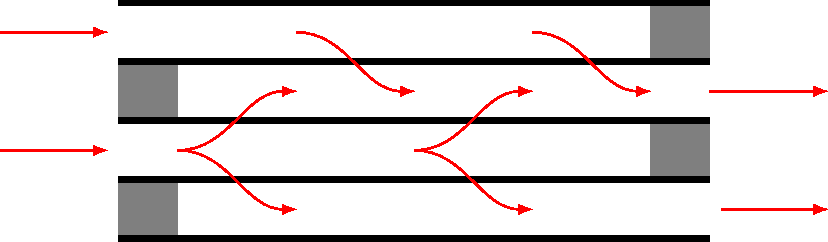
\includegraphics[width=\textwidth]{figures/wall_flow_DPF_figure.pdf}}
               {Kuvituskuva hiukkassuodattimen toiminnasta. Pakokaasu virtaa avoimiin putkiin ja kulkee seinämien läpi.}
    \caption{Pakokaasu virtaa suodattimessa huokoisten seinämien läpi. Yli 90\% pakokaasun hiukkasmassasta jää huokoisten seinämien sisään ja pinnalle.}
    \label{fig:wall-flow-dpf}
\end{figure}



\section{Regenerointi}
\begin{align*}
    \ce{C + 1/2 O2 &-> CO }\\
    \ce{C + O2 &-> CO2}\\
    \ce{C + NO2 &-> CO +  NO}  \\
    \ce{C + 2 NO2 &-> CO2 + 2 NO}  \\
    \ce{C + NO2 + 1/2 O2 &-> CO2 + NO}  \\
    \ce{C + NO2 + 1/2 O2 &-> CO + NO2} 
\end{align*}
\cite{LiuGuanlin2021Roio}


\section{Hiukkassuodattimen matemaattinen esitys}

\begin{figure}[H]
    \centering 
    \begin{tikzpicture}
    % Draw the first rectangle
    \node[draw, rectangle, minimum width=1.5cm, minimum height=3cm] (rect1) at (0, 0) {Rectangle 1};

    % Draw the second rectangle
    \node[draw, rectangle, minimum width=1.5cm, minimum height=3cm] (rect2) at (4, 0) {Rectangle 2};

    % Draw arrows between rectangles
    \draw[-{Latex}, thick] ([yshift=-0.5cm]rect1.north east) -- ([yshift=-0.5cm]rect2.north west);
    \draw[-{Latex}, thick] ([yshift=0.5cm]rect1.south east) -- ([yshift=0.5cm]rect2.south west);

    % Draw inputs to rect1
    \draw[-{Latex}, thick] (-3, 1) -- ([yshift=1cm]rect1.west) node[above left] {Nokilataus (g/l)};
    \draw[-{Latex}, thick] (-3, -1) -- ([yshift=-1cm]rect1.west) node[below left] {Tuhkalataus (g/l)};

    % Draw output from rect2
    \draw[-{Latex}, thick] (rect2.east) -- (7, 0) node[above right] {Paine (hPa)};

\end{tikzpicture}
    \caption{}
    \label{fig:blocks1}
\end{figure}

Painehäviö suodattimen sisäänmenossa
\begin{align}
    \Delta P_{inletch} = \frac{1}{6} \cdot
    \frac{\dot{m}}{\rho(T)} \cdot \mu(T) 
    \cdot F \cdot \frac{L^2}{V} \cdot \frac{(\alpha_{in}-\alpha_{out}+2 d_{wall})^2}{(\alpha_{in}-2d_{soot}-2d_{ash})^4}
    \label{eq:PDinletchannel}
\end{align}

Painehäviö suodattimen ulostulossa 
\begin{align}
    \Delta P_{outletopen} = \frac{1}{6} \cdot
    \frac{\dot{m}}{\rho(T)} \cdot \mu(T) 
    \cdot F \cdot \frac{L^2}{V} \cdot \frac{(\alpha_{in}-\alpha_{out}+2 d_{wall})^2}{\alpha_{out}^4}
    \label{eq:PDoutletopen}
\end{align}

Painehäviö suodattimen seinämillä
\begin{align}
    \Delta P_{filterwall} = \frac{1}{4} \cdot
    \frac{\dot{m}}{\rho(T)} \cdot \mu(T) 
    \cdot \frac{d_{wall}}
    {n_{open}\cdot L \cdot \kappa_{wall} \cdot \alpha_{out}}
    \label{eq:PDfilterwall}
\end{align}

Nokikerroksen aiheuttama painehäviö
\begin{align}
    \Delta P_{soot} =  \frac{1}{8} \cdot
    \frac{\dot{m}}{\rho(T)} \cdot \mu(T) \cdot 
    \frac{\ln{\frac{\alpha_{out}-2d_{ash}}{\alpha_{out}-2d_{soot}-2d_{ash}}}}
    {n_{open}\cdot L \cdot \kappa_{soot}}
    \label{eq:PDsootlayer}
\end{align}

Tuhkakerroksen aiheuttama painehäviö
\begin{align}
    \Delta P_{ash} = \frac{1}{8} \cdot
    \frac{\dot{m}}{\rho(T)} \cdot \mu(T) \cdot 
    \frac{\ln{\frac{\alpha_{out}}{\alpha_{out}-2d_{ash}}}}
    {n_{open}\cdot L \cdot \kappa_{ash}}
    \label{eq:PDashlayer}
\end{align}